In this section we report the results of $\WW$ cross-section measurements in 
different jet bin or final states. The measurements are performed in the 
dataset corresponding to an integrated luminosity of  $\intlumiEightTeV$.
The data driven background estimates are evaluated consistently for each jet bin.

\subsection{Measurements in the 0-Jet bin}

Table~\ref{tab:datayields_wwxsec_0j} shows the expected number of signal and background events,
as well as the signal acceptance and measured cross section in each lepton channel.
Table ~\ref{tab:datayields_wwxsec_0j_incl} shows the results including all lepton channels.
The kinematic distributions of the events selected are shown in Figures \ref{fig:xs_kinematics_mm_0j} - \ref{fig:xs_kinematics_incl_0j}.

\begin{table}[!ht]
{\small
\begin{center}
\begin{tabular}{|l|c|c|c|c|}
\hline
Sample  & mm    & me    & em    & ee    \\ \hline
$qqWW$  & $188.23 \pm 2.83 \pm 13.63 $  & $249.88 \pm 3.24 \pm 17.61 $  & $315.89 \pm 3.77 \pm 22.26 $  & $126.53 \pm 2.39 \pm 9.75 $   \\
$qqWW$  & $13.58 \pm 0.56 \pm 4.17 $    & $15.58 \pm 0.59 \pm 4.78 $    & $20.52 \pm 0.73 \pm 6.30 $    & $9.89 \pm 0.51 \pm 3.05 $ \\
$t\bar{t} + tW$ & $40.32 \pm 2.65 \pm 8.27 $    & $54.95 \pm 3.29 \pm 11.27 $   & $70.76 \pm 3.65 \pm 14.51 $   & $27.55 \pm 2.40 \pm 5.65 $    \\
$W+jets$    & $12.13 \pm 3.29 \pm 4.37 $    & $19.42 \pm 2.71 \pm 6.99 $    & $36.40 \pm 3.73 \pm 13.11 $   & $13.27 \pm 1.29 \pm 4.78 $    \\
$WZ$    & $7.40 \pm 0.23 \pm 0.84 $ & $5.88 \pm 0.21 \pm 0.66 $ & $9.71 \pm 0.27 \pm 1.09 $ & $4.32 \pm 0.18 \pm 0.50 $ \\
$ZZ$    & $6.09 \pm 0.18 \pm 0.60 $ & $0.24 \pm 0.03 \pm 0.02 $ & $0.37 \pm 0.03 \pm 0.04 $ & $4.13 \pm 0.15 \pm 0.42 $ \\
$Z/\gamma*$ & $36.25 \pm 6.79 \pm 10.65 $   & $0.16 \pm 0.16 \pm 0.02 $ & $1.24 \pm 0.50 \pm 0.12 $ & $23.23 \pm 6.62 \pm 6.82 $    \\
$W\gamma*/W+\gamma$ & $0.52 \pm 0.19 \pm 0.16 $ & $3.26 \pm 1.19 \pm 0.98 $ & $6.41 \pm 1.50 \pm 1.92 $ & $18.39 \pm 3.76 \pm 5.52 $    \\
\hline \hline
Total B.    & $102.72 \pm 8.00 \pm 14.21 $  & $83.91 \pm 4.43 \pm 13.31 $   & $124.90 \pm 5.46 \pm 19.67 $  & $90.89 \pm 8.09 \pm 11.50 $   \\ \hline \hline
Total B.+S. & $304.52 \pm 8.51 \pm 20.13 $  & $349.36 \pm 5.52 \pm 22.59 $  & $461.30 \pm 6.68 \pm 30.37 $  & $227.32 \pm 8.45 \pm 15.38 $  \\ \hline \hline
Data    & $360$     & $428$     & $549$     & $205$     \\ \hline \hline
Acceptance ( \% )   & $0.66 \pm 0.05    $& $0.87 \pm 0.07   $& $1.10 \pm 0.09   $& $0.45 \pm 0.04   $\\
Cross Section ( pb )    & $72.81 \pm 5.37 \pm 7.40$     & $74.03 \pm 4.45 \pm 6.49$     & $72.00 \pm 3.98 \pm 6.57$     & $47.77 \pm 5.99 \pm 7.12$     \\ \hline
\end{tabular}
\caption{Summary of yields for 0-jet channel.Uncertainties on yields and cross sections are $\mathrm{(stat.)} \pm \mathrm{(syst.)}$. The systematic uncertainty on the cross section does not include the luminosity}
\label{tab:datayields_wwxsec_0j}
\end{center}}
\end{table}

\begin{table}[!ht]
{\small
\begin{center}
\begin{tabular}{|l|c|c|c|c|}
\hline
Sample  & incl  \\ \hline
$qqWW$  & $880.53 \pm 6.20 \pm 63.26 $  \\
$qqWW$  & $59.56 \pm 1.21 \pm 18.31 $   \\
$t\bar{t} + tW$ & $193.59 \pm 6.08 \pm 39.69 $  \\
$W+jets$    & $81.22 \pm 5.81 \pm 29.24 $   \\
$WZ$    & $27.31 \pm 0.46 \pm 3.08 $    \\
$ZZ$    & $10.83 \pm 0.24 \pm 1.08 $    \\
$Z/\gamma*$ & $60.88 \pm 9.50 \pm 17.48 $   \\
$W\gamma*/W+\gamma$ & $28.58 \pm 4.22 \pm 8.57 $    \\
\hline \hline
Total B.    & $402.41 \pm 13.38 \pm 53.10 $ \\ \hline \hline
Total B.+S. & $1342.50 \pm 14.79 \pm 84.59 $    \\ \hline \hline
Data    & $1542$    \\ \hline \hline
Acceptance ( \% )   & $3.08 \pm 0.24    $\\
Cross Section ( pb )    & $69.23 \pm 2.39 \pm 6.40$     \\ \hline
\end{tabular}
\caption{Summary of yields for 0-jet channel.Uncertainties on yields and cross sections are $\mathrm{(stat.)} \pm \mathrm{(syst.)}$. The systematic uncertainty on the cross section does not include the luminosity}
\label{tab:datayields_wwxsec_0j_incl}
\end{center}}
\end{table}

\begin{figure}[!hbtp]
\centering
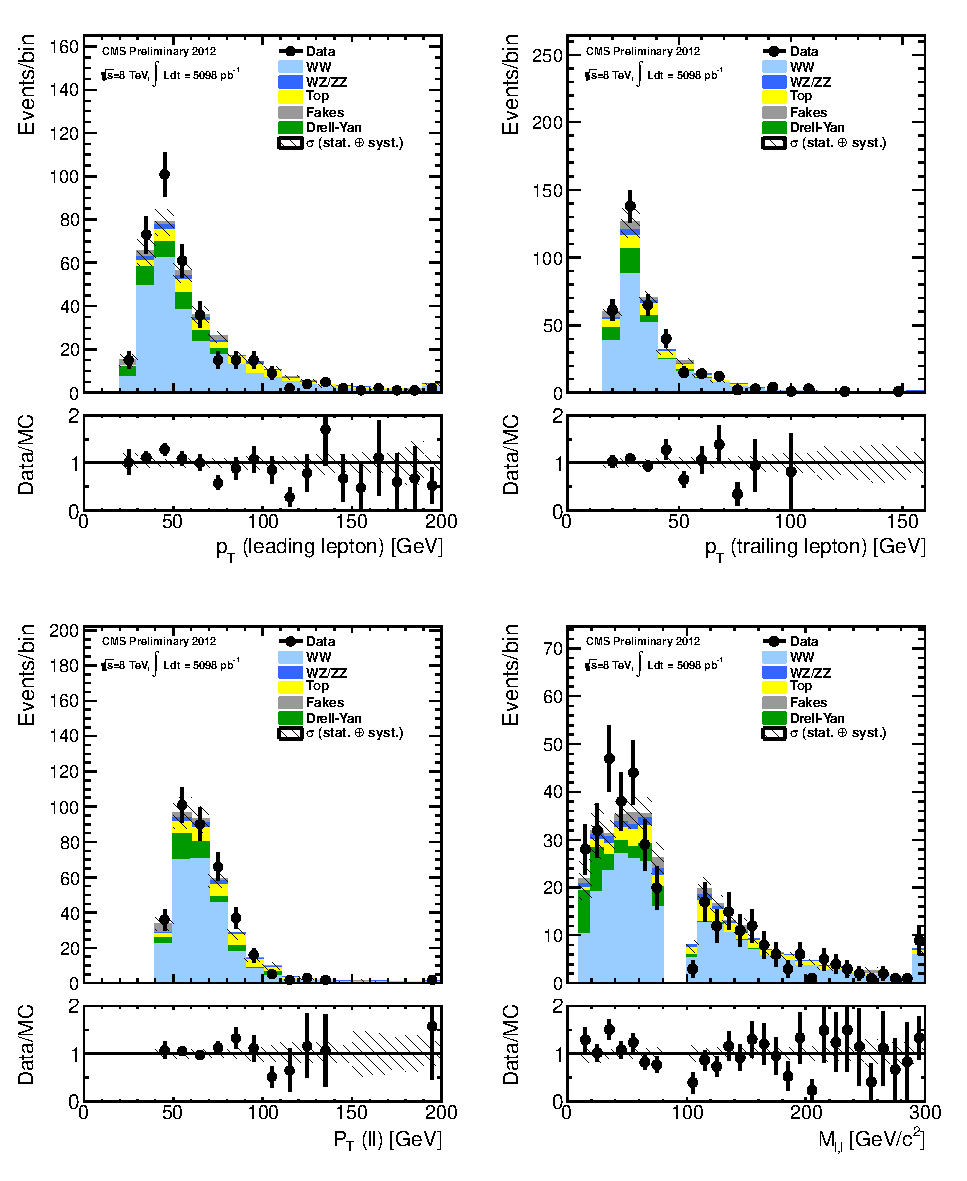
\includegraphics[width=1\textwidth]{figures/ww_analysis20_0_ALL_mm_0j.pdf} %FIXME
\caption{Kinematic distributions in the $\mu\mu$ final state in the 0-jet bin.
The WW component has been scaled to the cross section measured in the 0-jet bin.}
\label{fig:xs_kinematics_mm_0j}
\end{figure}
\begin{figure}[!hbtp]
\centering
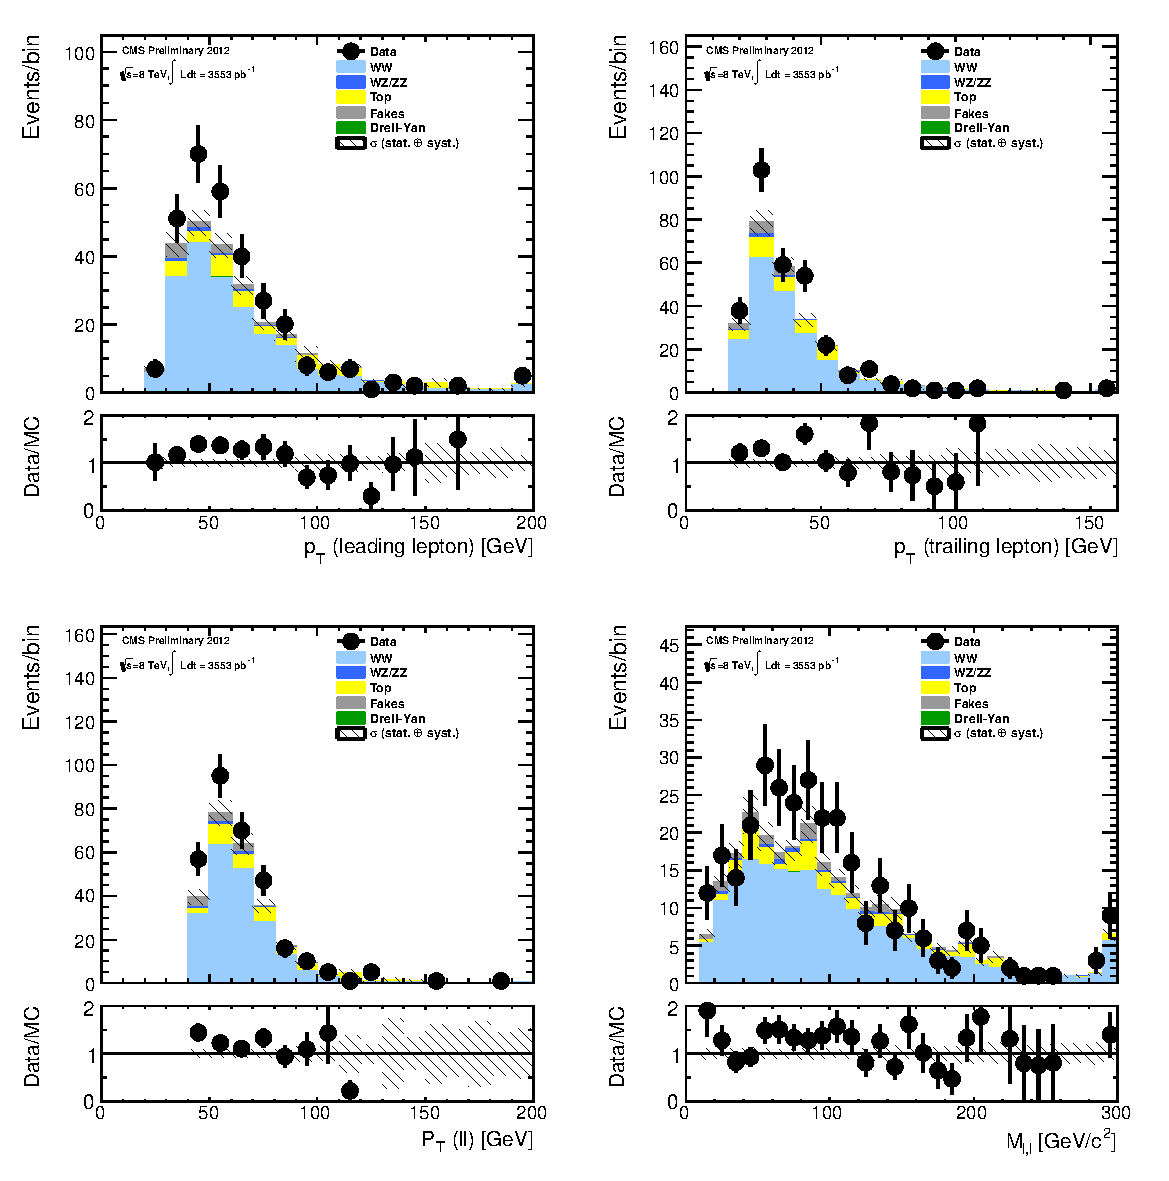
\includegraphics[width=1\textwidth]{figures/ww_analysis20_0_ALL_me_0j.pdf} %FIXME
\caption{Kinematic distributions in the $\mu e$ final state in the 0-jet bin.
The WW component has been scaled to the cross section measured in the 0-jet bin.}
\label{fig:xs_kinematics_me_0j}
\end{figure}
\begin{figure}[!hbtp]
\centering
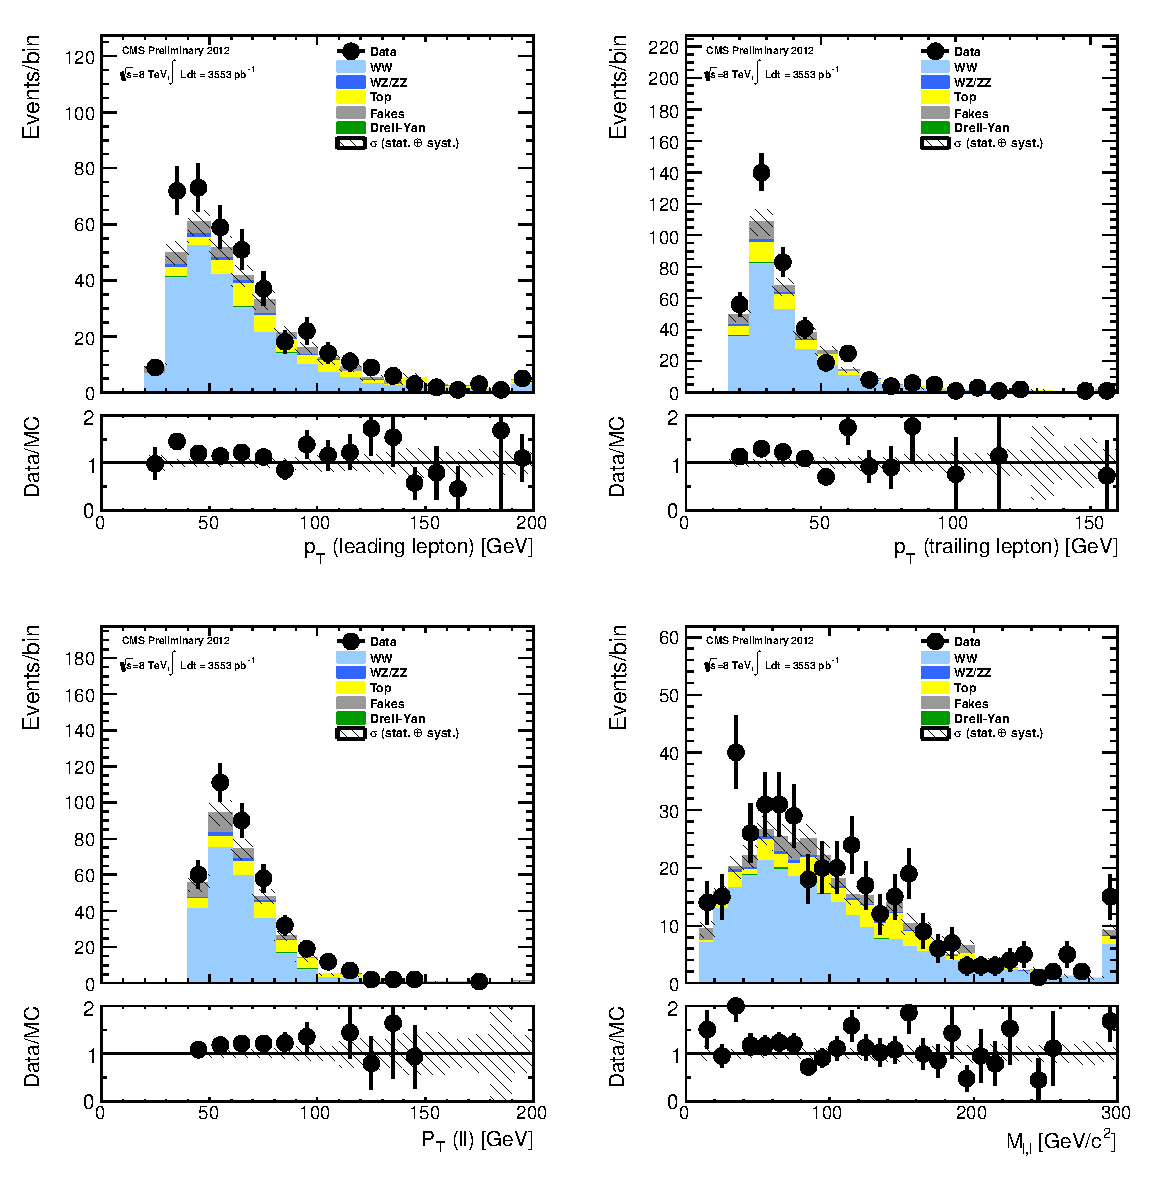
\includegraphics[width=1\textwidth]{figures/ww_analysis20_0_ALL_em_0j.pdf} %FIXME
\caption{Kinematic distributions in the $e\mu$ final state in the 0-jet bin.
The WW component has been scaled to the cross section measured in the 0-jet bin.}
\label{fig:xs_kinematics_em_0j}
\end{figure}
\begin{figure}[!hbtp]
\centering
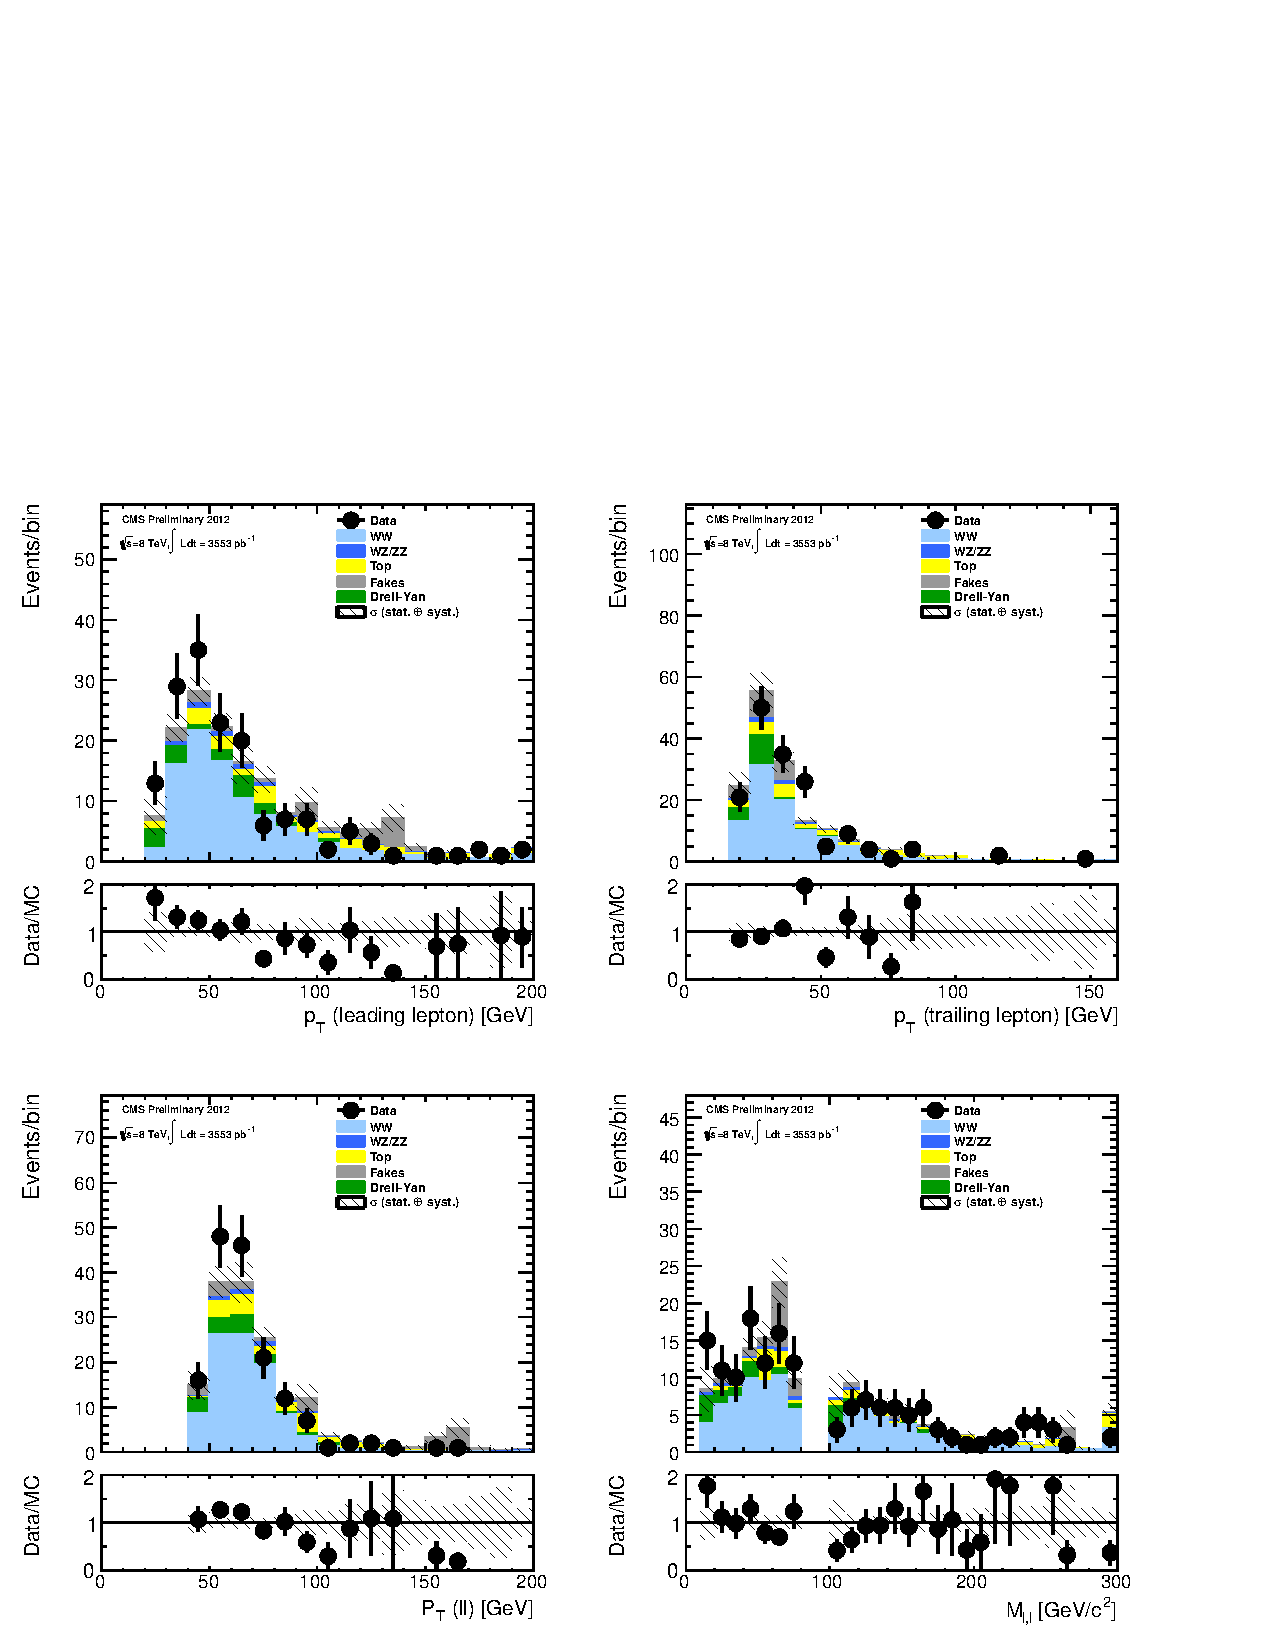
\includegraphics[width=1\textwidth]{figures/ww_analysis20_0_ALL_ee_0j.pdf} %FIXME
\caption{Kinematic distributions in the $ee$ final state in the 0-jet bin.
The WW component has been scaled to the cross section measured in the 0-jet bin.}
\label{fig:xs_kinematics_ee_0j}
\end{figure}
\begin{figure}[!hbtp]
\centering
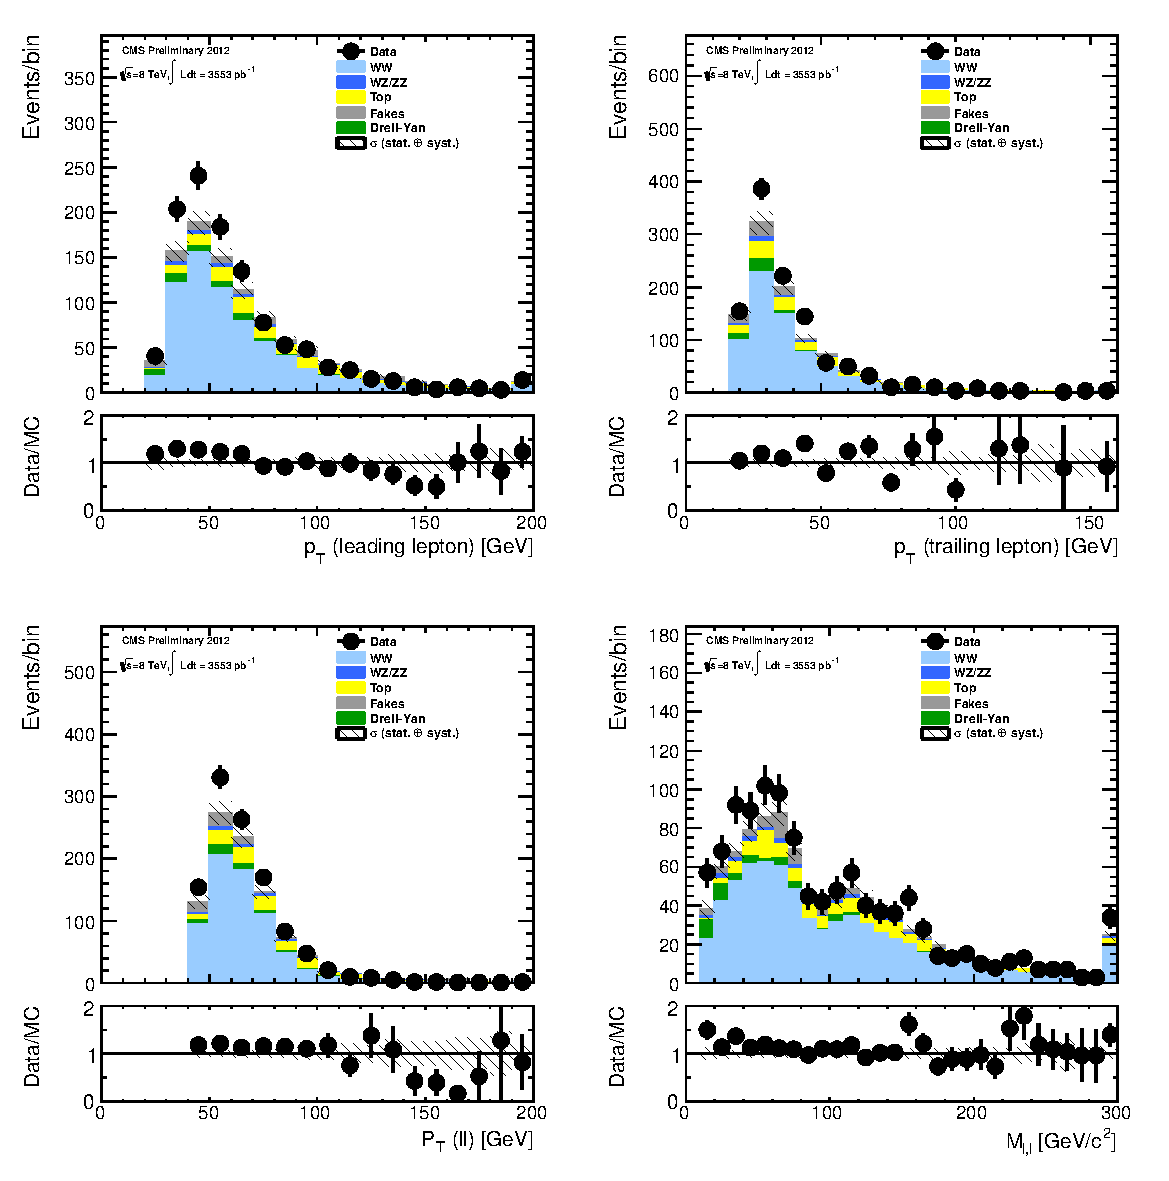
\includegraphics[width=1\textwidth]{figures/ww_analysis20_0_ALL_incl_0j.pdf} %FIXME
\caption{Kinematic distributions in the inclusive final state in the 0-jet bin.
The WW component has been scaled to the cross section measured in the 0-jet bin.}
\label{fig:xs_kinematics_incl_0j}
\end{figure}

\clearpage
\subsection{Measurements in the 1-Jet bin}

Table~\ref{tab:datayields_wwxsec_1j} shows the expected number of signal and background events,
as well as the signal acceptance and measured cross section in each lepton channel.
Table ~\ref{tab:datayields_wwxsec_1j_incl} shows the results including all lepton channels.
The kinematic distributions of the events selected are shown in Figures \ref{fig:xs_kinematics_mm_1j} - \ref{fig:xs_kinematics_incl_1j}.

\begin{table}[!ht]
{\small
\begin{center}
\begin{tabular}{|l|c|c|c|c|}
\hline
Sample  & mm    & me    & em    & ee    \\ \hline
$qqWW$  & $61.21 \pm 1.58 \pm 4.43 $    & $109.55 \pm 2.20 \pm 7.72 $   & $134.63 \pm 2.46 \pm 9.49 $   & $41.70 \pm 1.34 \pm 3.21 $    \\
$qqWW$  & $3.94 \pm 0.31 \pm 1.21 $ & $6.00 \pm 0.37 \pm 1.84 $ & $6.59 \pm 0.38 \pm 2.02 $ & $3.38 \pm 0.31 \pm 1.04 $ \\
$t\bar{t} + tW$ & $94.23 \pm 3.41 \pm 5.18 $    & $147.40 \pm 4.34 \pm 8.11 $   & $173.80 \pm 4.33 \pm 9.56 $   & $57.79 \pm 2.57 \pm 3.18 $    \\
$W+jets$    & $9.38 \pm 3.17 \pm 3.38 $ & $19.51 \pm 3.36 \pm 7.02 $    & $31.61 \pm 3.97 \pm 11.38 $   & $6.05 \pm 0.96 \pm 2.18 $ \\
$WZ$    & $3.91 \pm 0.17 \pm 0.44 $ & $6.85 \pm 0.23 \pm 0.77 $ & $11.17 \pm 0.30 \pm 1.25 $    & $4.09 \pm 0.22 \pm 0.48 $ \\
$ZZ$    & $2.09 \pm 0.11 \pm 0.20 $ & $0.22 \pm 0.02 \pm 0.02 $ & $0.39 \pm 0.03 \pm 0.04 $ & $1.22 \pm 0.08 \pm 0.12 $ \\
$Z/\gamma*$ & $48.14 \pm 9.13 \pm 6.27 $    & $14.25 \pm 5.16 \pm 1.43 $    & $9.54 \pm 2.82 \pm 0.95 $ & $39.46 \pm 9.69 \pm 5.14 $    \\
$W\gamma*/W+\gamma$ & $0.03 \pm 0.03 \pm 0.01 $ & $2.33 \pm 1.24 \pm 0.70 $ & $8.75 \pm 3.03 \pm 2.63 $ & $6.00 \pm 1.31 \pm 1.80 $ \\
\hline \hline
Total B.    & $157.77 \pm 10.25 \pm 8.82 $  & $190.56 \pm 7.64 \pm 10.87 $  & $235.26 \pm 7.19 \pm 15.17 $  & $114.61 \pm 10.16 \pm 6.69 $  \\ \hline \hline
Total B.+S. & $222.92 \pm 10.38 \pm 9.95 $  & $306.11 \pm 7.96 \pm 13.46 $  & $376.47 \pm 7.61 \pm 18.01 $  & $159.69 \pm 10.25 \pm 7.49 $  \\ \hline \hline
Data    & $249$     & $309$     & $397$     & $153$     \\ \hline \hline
Acceptance ( \% )   & $0.21 \pm 0.02    $& $0.38 \pm 0.03   $& $0.46 \pm 0.04   $& $0.15 \pm 0.01   $\\
Cross Section ( pb )    & $79.97 \pm 13.83 \pm 13.45$   & $58.54 \pm 8.69 \pm 7.98$     & $65.41 \pm 8.06 \pm 8.48$     & $48.64 \pm 15.67 \pm 15.94$   \\ \hline
\end{tabular}
\caption{Summary of yields for 1-jet channel.Uncertainties on yields and cross sections are $\mathrm{(stat.)} \pm \mathrm{(syst.)}$. The systematic uncertainty on the cross section does not include the luminosity}
\label{tab:datayields_wwxsec_1j}
\end{center}}
\end{table}
\begin{table}[!ht]
{\small
\begin{center}
\begin{tabular}{|l|c|c|c|c|}
\hline
Sample  & incl  \\ \hline
$qqWW$  & $347.09 \pm 3.90 \pm 24.86 $  \\
$qqWW$  & $19.90 \pm 0.69 \pm 6.12 $    \\
$t\bar{t} + tW$ & $473.21 \pm 7.47 \pm 26.03 $  \\
$W+jets$    & $66.55 \pm 6.17 \pm 23.96 $   \\
$WZ$    & $26.01 \pm 0.47 \pm 2.93 $    \\
$ZZ$    & $3.92 \pm 0.14 \pm 0.39 $ \\
$Z/\gamma*$ & $111.39 \pm 14.55 \pm 11.65 $ \\
$W\gamma*/W+\gamma$ & $17.11 \pm 3.52 \pm 5.13 $    \\
\hline \hline
Total B.    & $698.21 \pm 17.84 \pm 37.71 $ \\ \hline \hline
Total B.+S. & $1065.20 \pm 18.28 \pm 45.58 $    \\ \hline \hline
Data    & $1108$    \\ \hline \hline
Acceptance ( \% )   & $1.20 \pm 0.09    $\\
Cross Section ( pb )    & $63.77 \pm 5.18 \pm 8.21$     \\ \hline
\end{tabular}
\caption{Summary of yields for 1-jet channel.Uncertainties on yields and cross sections are $\mathrm{(stat.)} \pm \mathrm{(syst.)}$. The systematic uncertainty on the cross section does not include the luminosity}
\label{tab:datayields_wwxsec_1j_incl}
\end{center}}
\end{table}

\begin{figure}[!hbtp]
\centering
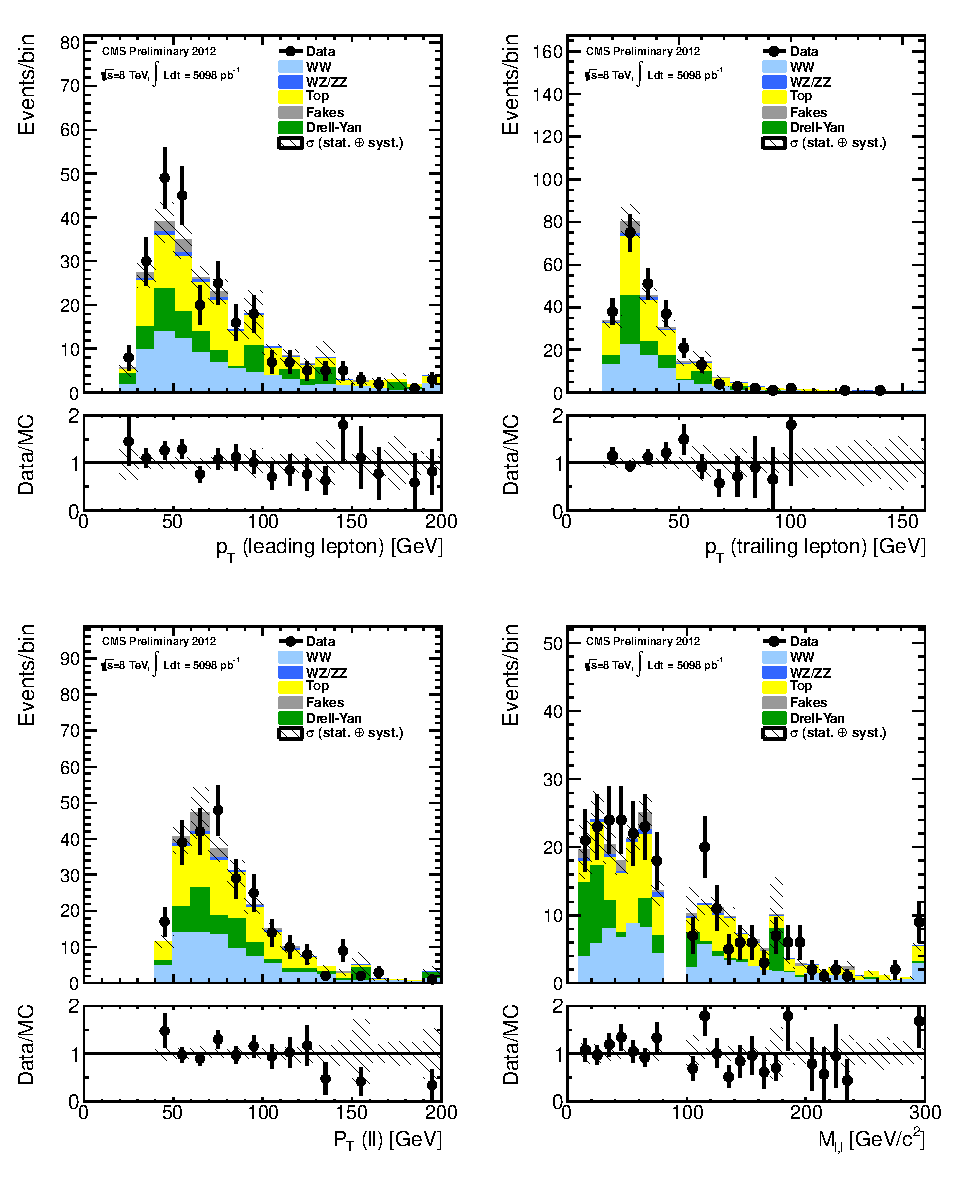
\includegraphics[width=1\textwidth]{figures/ww_analysis20_0_ALL_mm_1j.pdf} %FIXME
\caption{Kinematic distributions in the $\mu\mu$ final state in the 1-jet bin.
The WW component has been scaled to the cross section measured in the 0-jet bin.}
\label{fig:xs_kinematics_mm_1j}
\end{figure}
\begin{figure}[!hbtp]
\centering
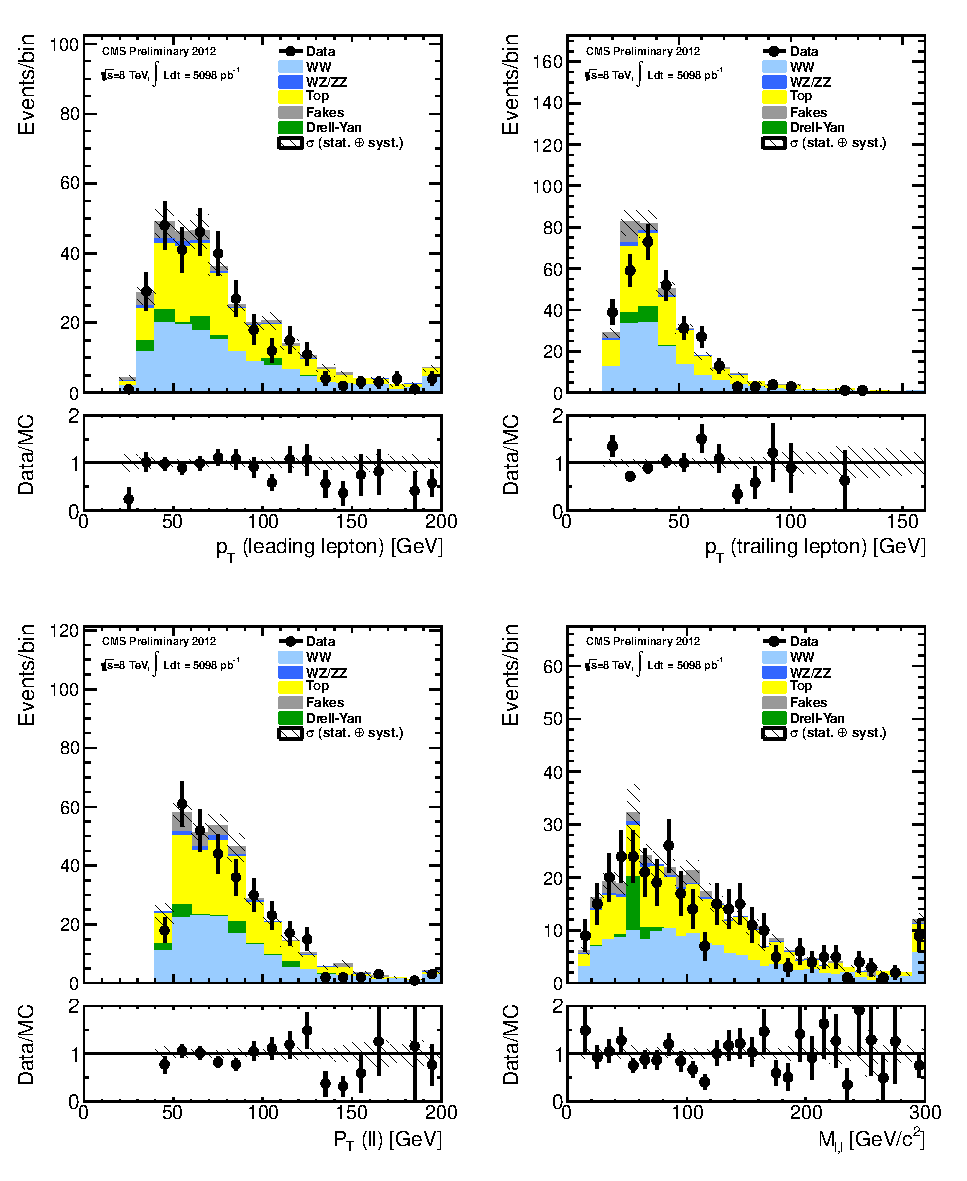
\includegraphics[width=1\textwidth]{figures/ww_analysis20_0_ALL_me_1j.pdf} %FIXME
\caption{Kinematic distributions in the $\mu e$ final state in the 1-jet bin.
The WW component has been scaled to the cross section measured in the 0-jet bin.}
\label{fig:xs_kinematics_me_1j}
\end{figure}
\begin{figure}[!hbtp]
\centering
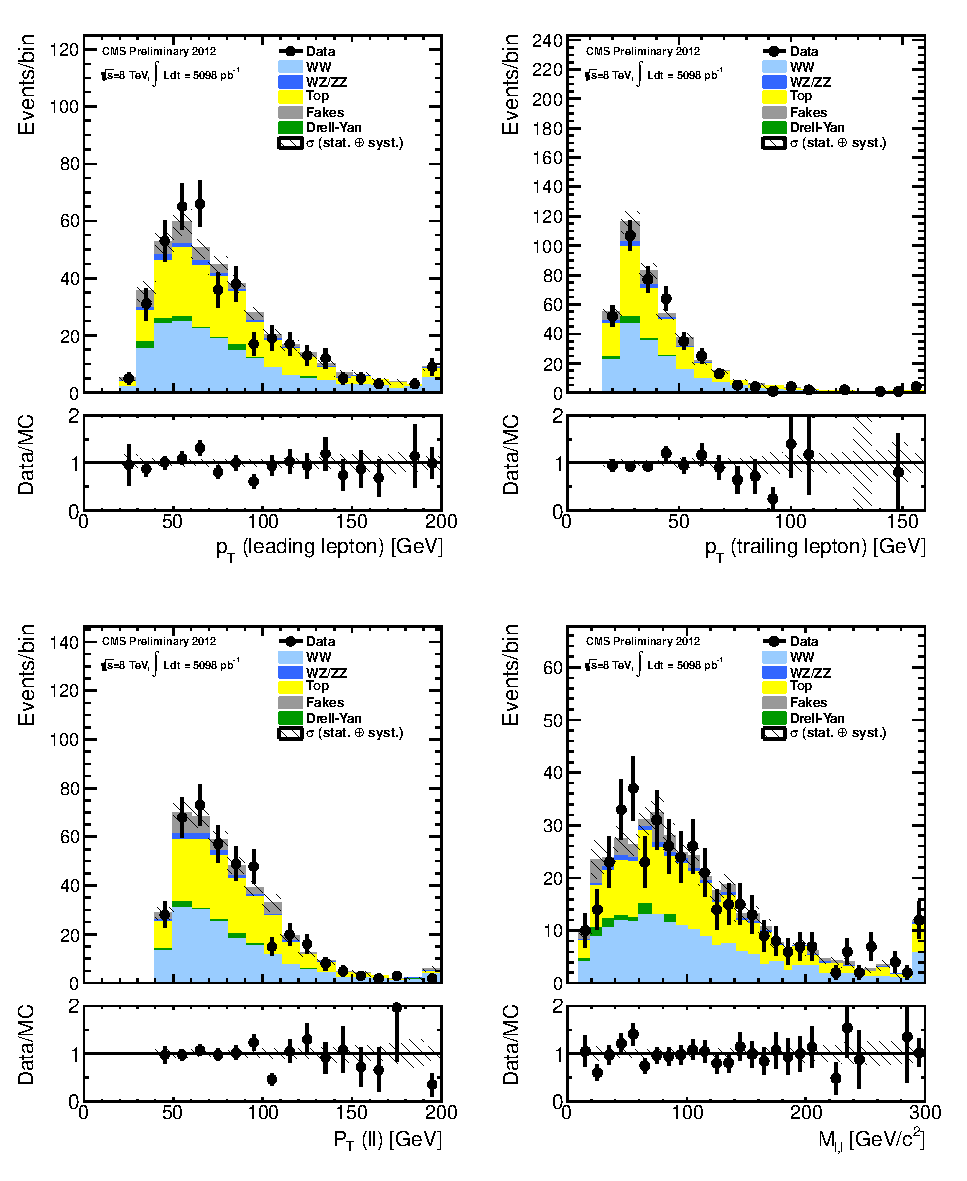
\includegraphics[width=1\textwidth]{figures/ww_analysis20_0_ALL_em_1j.pdf} %FIXME
\caption{Kinematic distributions in the $e\mu$ final state in the 1-jet bin.
The WW component has been scaled to the cross section measured in the 0-jet bin.}
\label{fig:xs_kinematics_em_1j}
\end{figure}
\begin{figure}[!hbtp]
\centering
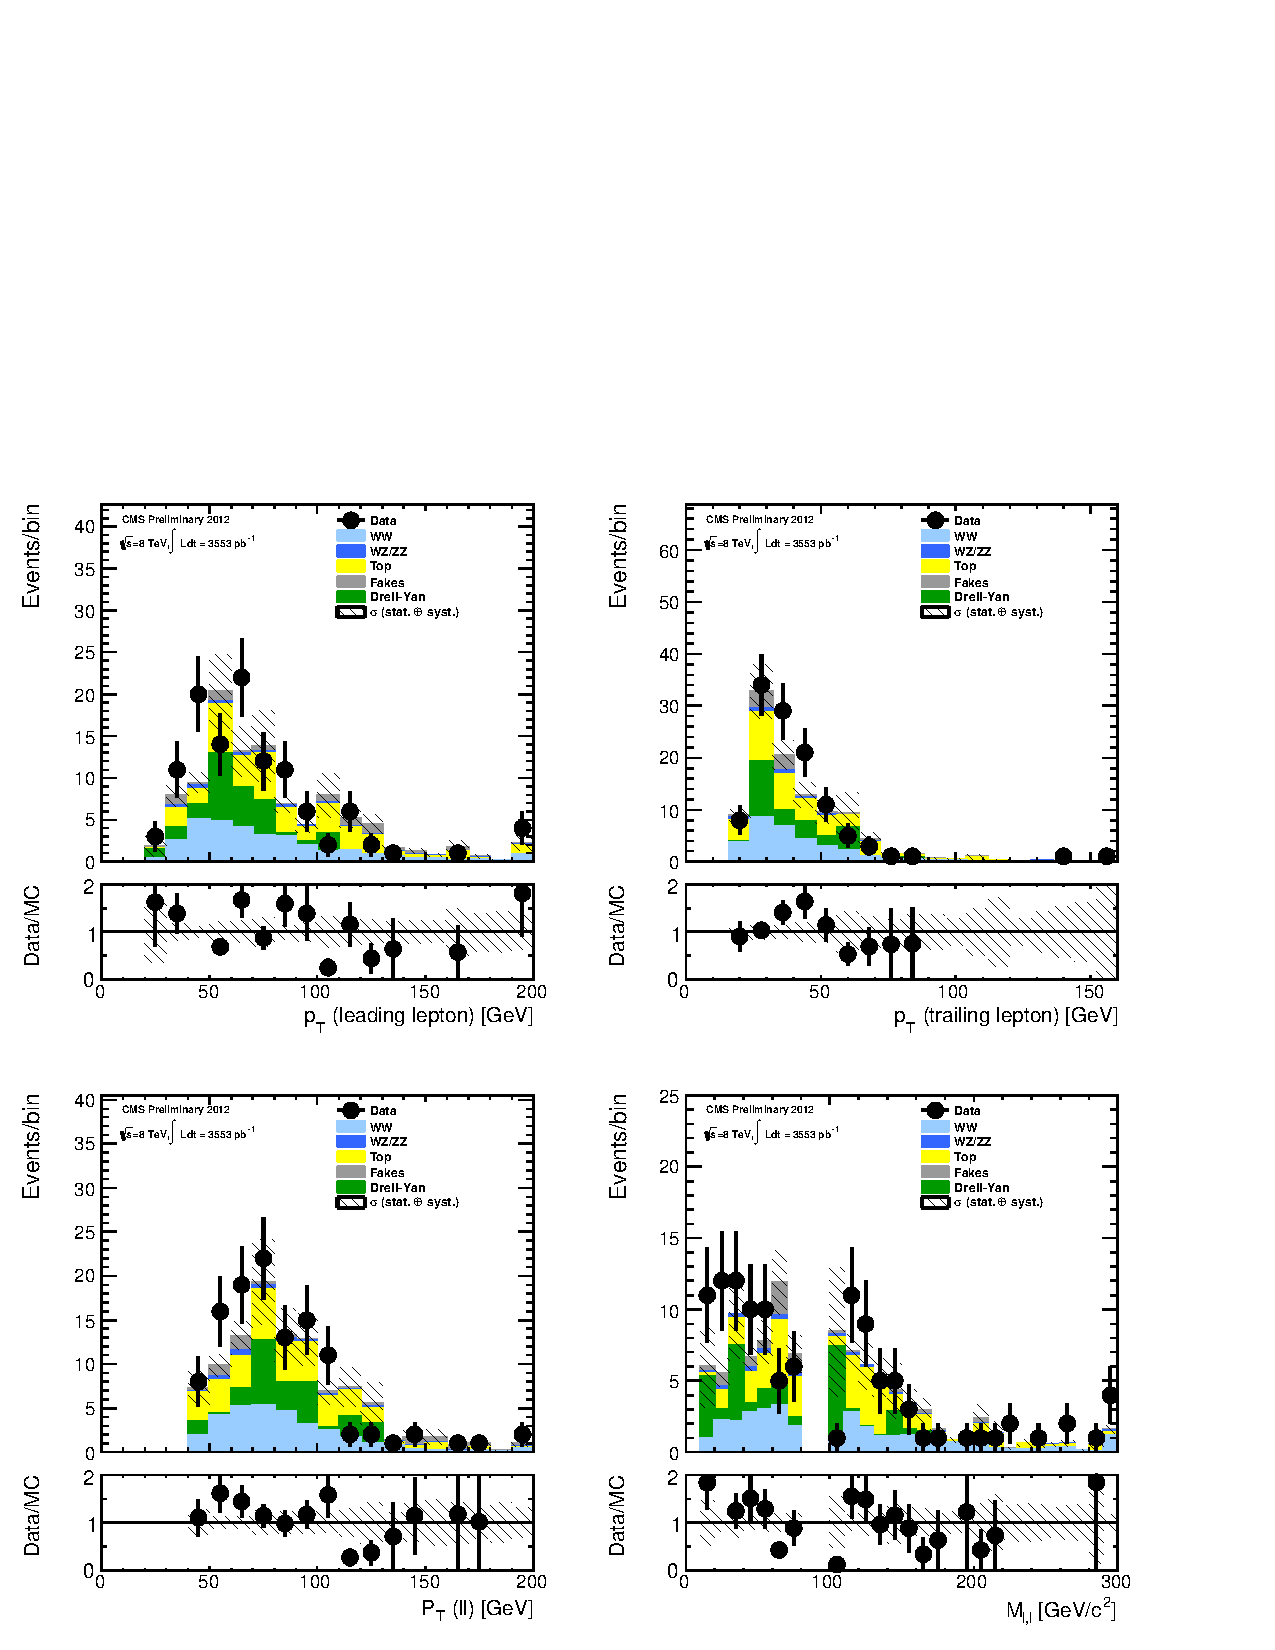
\includegraphics[width=1\textwidth]{figures/ww_analysis20_0_ALL_ee_1j.pdf} %FIXME
\caption{Kinematic distributions in the $ee$ final state in the 1-jet bin.
The WW component has been scaled to the cross section measured in the 0-jet bin.}
\label{fig:xs_kinematics_ee_1j}
\end{figure}
\begin{figure}[!hbtp]
\centering
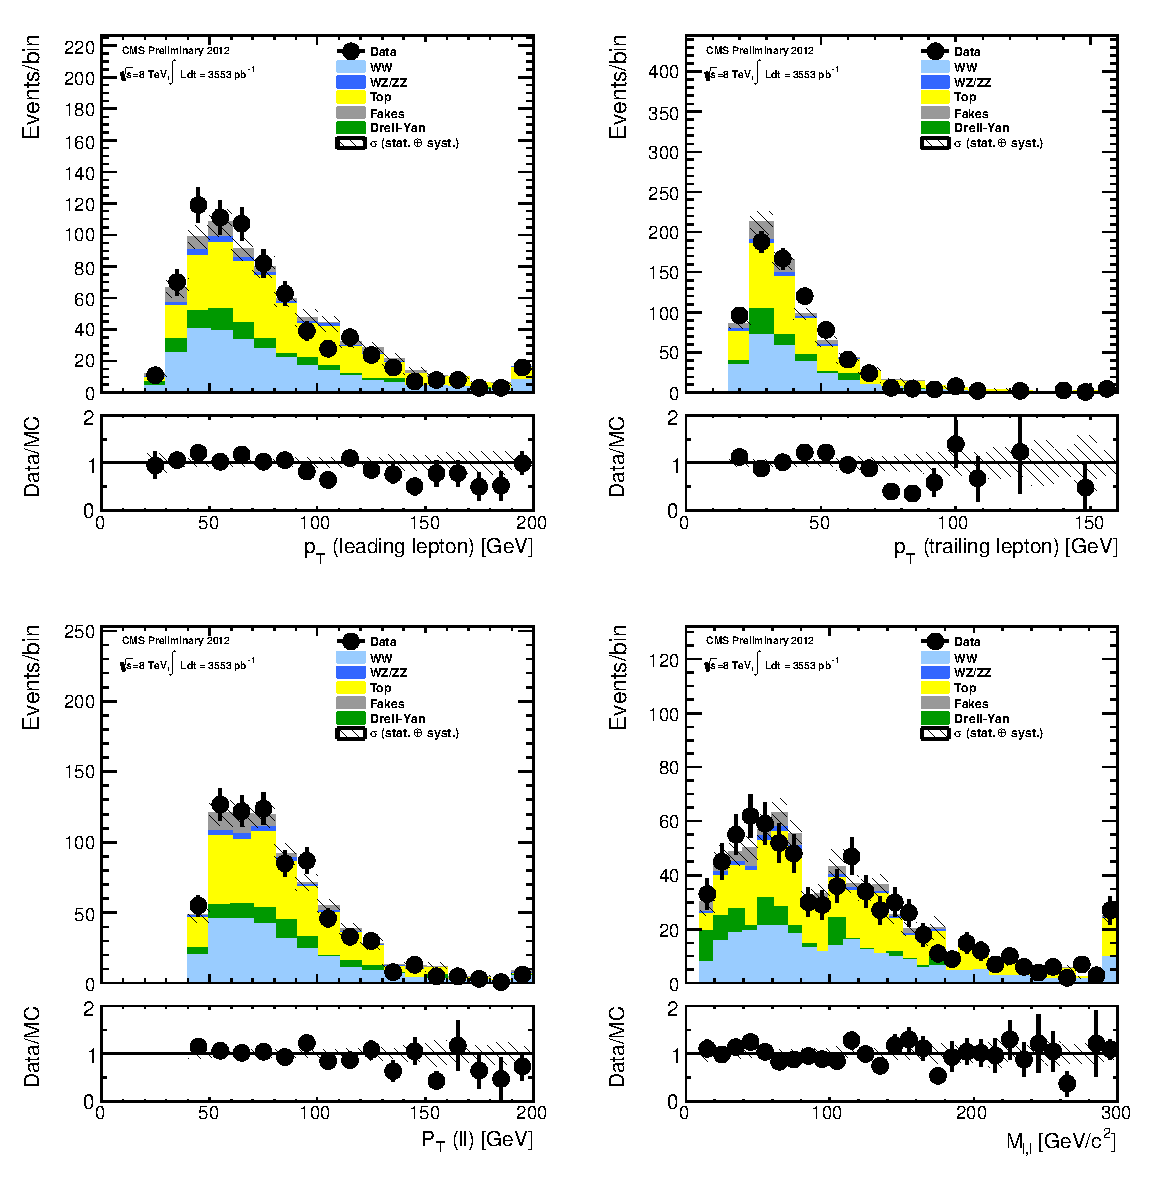
\includegraphics[width=1\textwidth]{figures/ww_analysis20_0_ALL_incl_1j.pdf} %FIXME
\caption{Kinematic distributions in the inclusive final state in the 1-jet bin.
The WW component has been scaled to the cross section measured in the 0-jet bin.}
\label{fig:xs_kinematics_incl_1j}
\end{figure}

\clearpage
\subsection{Measurements in the 2-Jet bin}

Table~\ref{tab:datayields_wwxsec_2j} shows the expected number of signal and background events,
as well as the signal acceptance and measured cross section in each lepton channel.
Table ~\ref{tab:datayields_wwxsec_2j_incl} shows the results including all lepton channels.
The kinematic distributions of the events selected are shown in Figures \ref{fig:xs_kinematics_mm_2j} - \ref{fig:xs_kinematics_incl_2j}.
\begin{table}[!ht]
{\small
\begin{center}
\begin{tabular}{|l|c|c|c|c|}
\hline
Sample  & mm    & me    & em    & ee    \\ \hline
$qqWW$  & $28.67 \pm 1.08 \pm 2.08 $    & $42.16 \pm 1.33 \pm 2.97 $    & $52.13 \pm 1.56 \pm 3.67 $    & $19.64 \pm 0.93 \pm 1.51 $    \\
$qqWW$  & $0.55 \pm 0.10 \pm 0.17 $ & $1.22 \pm 0.17 \pm 0.38 $ & $1.32 \pm 0.19 \pm 0.41 $ & $0.72 \pm 0.15 \pm 0.22 $ \\
$t\bar{t} + tW$ & $139.00 \pm 3.77 \pm 7.92 $   & $170.51 \pm 3.29 \pm 9.72 $   & $207.88 \pm 3.75 \pm 11.85 $  & $89.35 \pm 2.66 \pm 5.09 $    \\
$W+jets$    & $10.85 \pm 3.52 \pm 3.91 $    & $12.26 \pm 2.67 \pm 4.41 $    & $17.32 \pm 3.17 \pm 6.24 $    & $3.85 \pm 0.88 \pm 1.39 $ \\
$WZ$    & $3.14 \pm 0.19 \pm 0.36 $ & $3.58 \pm 0.17 \pm 0.40 $ & $5.26 \pm 0.20 \pm 0.59 $ & $3.16 \pm 0.18 \pm 0.37 $ \\
$ZZ$    & $1.03 \pm 0.08 \pm 0.10 $ & $0.11 \pm 0.01 \pm 0.01 $ & $0.26 \pm 0.04 \pm 0.03 $ & $0.59 \pm 0.05 \pm 0.06 $ \\
$Z/\gamma*$ & $100.29 \pm 12.81 \pm 13.56 $ & $11.63 \pm 4.74 \pm 1.16 $    & $9.07 \pm 3.58 \pm 0.91 $ & $78.72 \pm 15.83 \pm 10.64 $  \\
$W\gamma*/W+\gamma$ & $0.00 \pm 0.00 \pm 0.00 $ & $0.53 \pm 0.42 \pm 0.16 $ & $1.27 \pm 0.97 \pm 0.38 $ & $1.27 \pm 0.69 \pm 0.38 $ \\
\hline \hline
Total B.    & $254.32 \pm 13.82 \pm 16.19 $ & $198.62 \pm 6.38 \pm 10.75 $  & $241.06 \pm 6.16 \pm 13.44 $  & $176.94 \pm 16.09 \pm 11.89 $ \\ \hline \hline
Total B.+S. & $283.54 \pm 13.86 \pm 16.32 $ & $242.01 \pm 6.51 \pm 11.16 $  & $294.51 \pm 6.35 \pm 13.94 $  & $197.29 \pm 16.12 \pm 11.99 $ \\ \hline \hline
Data    & $286$     & $254$     & $313$     & $185$     \\ \hline \hline
Acceptance ( \% )   & $0.10 \pm 0.01    $& $0.14 \pm 0.01   $& $0.17 \pm 0.01   $& $0.07 \pm 0.01   $\\
Cross Section ( pb )    & $61.91 \pm 33.05 \pm 41.87$   & $72.89 \pm 20.98 \pm 17.39$   & $76.87 \pm 18.90 \pm 16.88$   & $22.62 \pm 38.16 \pm 56.17$   \\ \hline
\end{tabular}
\caption{Summary of yields for 2-jet channel.Uncertainties on yields and cross sections are $\mathrm{(stat.)} \pm \mathrm{(syst.)}$. The systematic uncertainty on the cross section does not include the luminosity}
\label{tab:datayields_wwxsec_2j}
\end{center}}
\end{table}
\begin{table}[!ht]
{\small
\begin{center}
\begin{tabular}{|l|c|c|c|c|}
\hline
Sample  & incl  \\ \hline
$qqWW$  & $142.60 \pm 2.50 \pm 10.23 $  \\
$qqWW$  & $3.82 \pm 0.31 \pm 1.17 $ \\
$t\bar{t} + tW$ & $606.74 \pm 6.80 \pm 34.58 $  \\
$W+jets$    & $44.28 \pm 5.51 \pm 15.94 $   \\
$WZ$    & $15.14 \pm 0.37 \pm 1.71 $    \\
$ZZ$    & $2.00 \pm 0.11 \pm 0.20 $ \\
$Z/\gamma*$ & $199.70 \pm 21.22 \pm 24.29 $ \\
$W\gamma*/W+\gamma$ & $3.07 \pm 1.26 \pm 0.92 $ \\
\hline \hline
Total B.    & $870.94 \pm 22.99 \pm 45.21 $ \\ \hline \hline
Total B.+S. & $1017.36 \pm 23.13 \pm 46.37 $    \\ \hline \hline
Data    & $1038$    \\ \hline \hline
Acceptance ( \% )   & $0.48 \pm 0.04    $\\
Cross Section ( pb )    & $65.16 \pm 12.57 \pm 20.44$   \\ \hline
\end{tabular}
\caption{Summary of yields for 2-jet channel.Uncertainties on yields and cross sections are $\mathrm{(stat.)} \pm \mathrm{(syst.)}$. The systematic uncertainty on the cross section does not include the luminosity}
\label{tab:datayields_wwxsec_2j_incl}
\end{center}}
\end{table}

\begin{figure}[!hbtp]
\centering
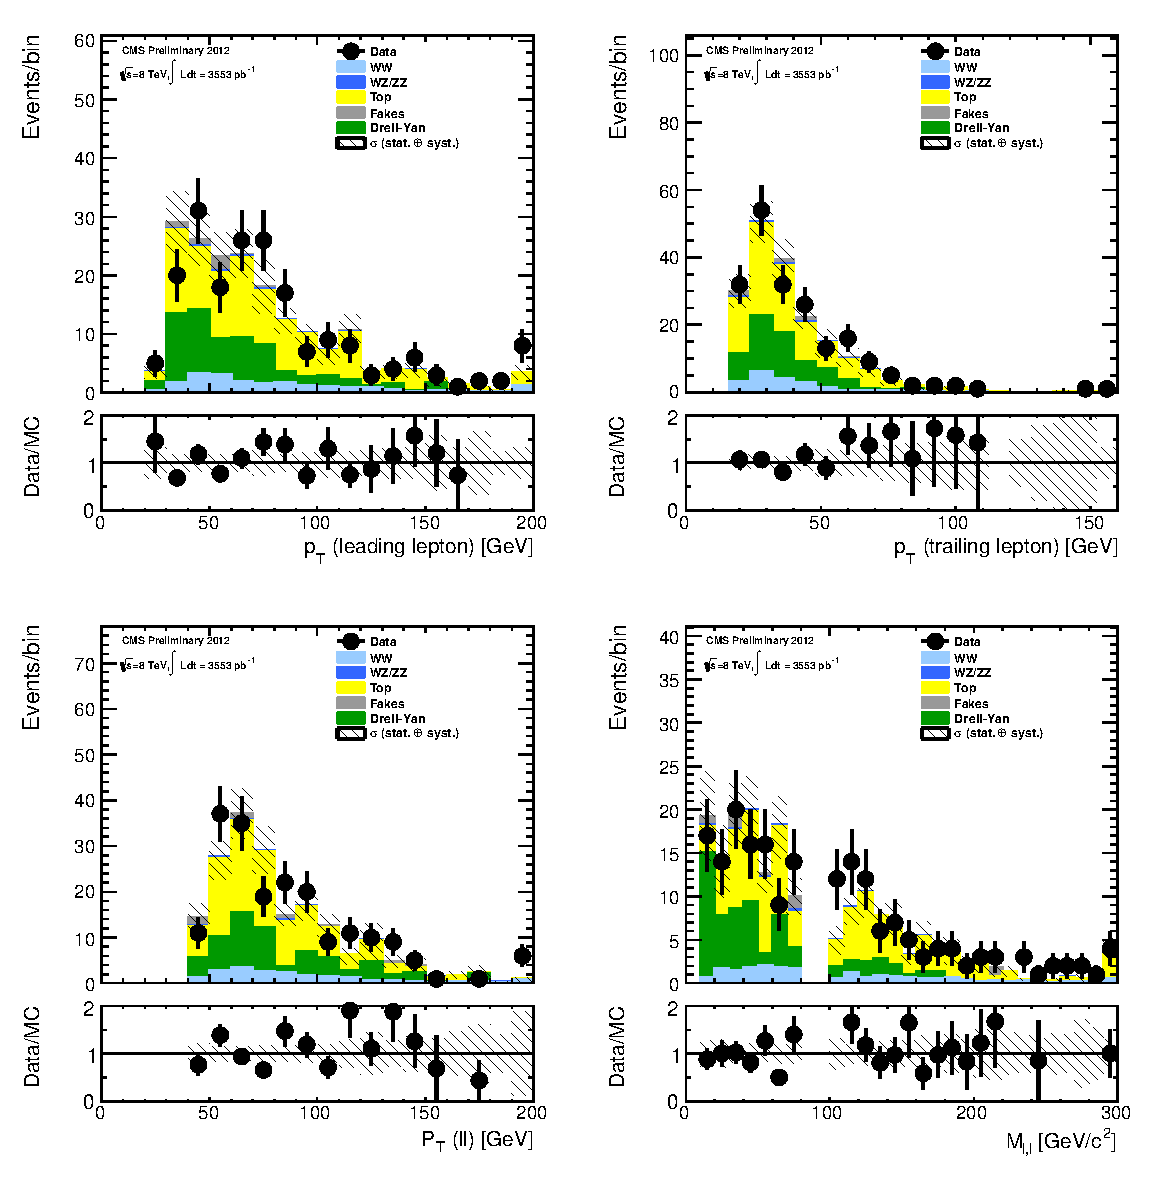
\includegraphics[width=1\textwidth]{figures/ww_analysis20_0_ALL_mm_2j.pdf} %FIXME
\caption{Kinematic distributions in the $\mu\mu$ final state in the 2-jet bin.
The WW component has been scaled to the cross section measured in the 0-jet bin.}
\label{fig:xs_kinematics_mm_2j}
\end{figure}
\begin{figure}[!hbtp]
\centering
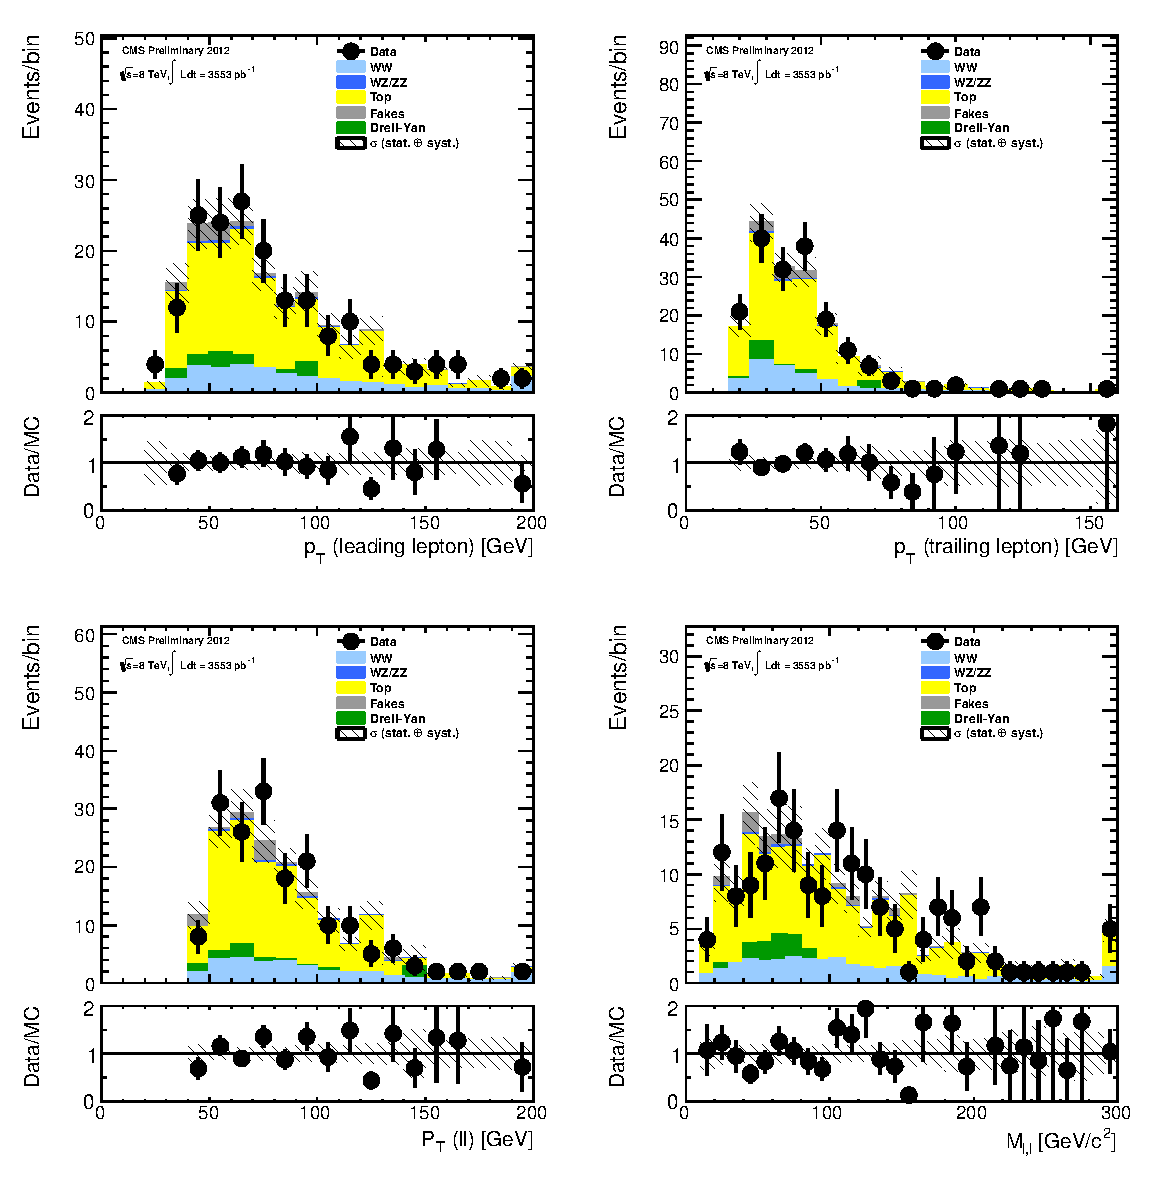
\includegraphics[width=1\textwidth]{figures/ww_analysis20_0_ALL_me_2j.pdf} %FIXME
\caption{Kinematic distributions in the $\mu e$ final state in the 2-jet bin.
The WW component has been scaled to the cross section measured in the 0-jet bin.}
\label{fig:xs_kinematics_me_2j}
\end{figure}
\begin{figure}[!hbtp]
\centering
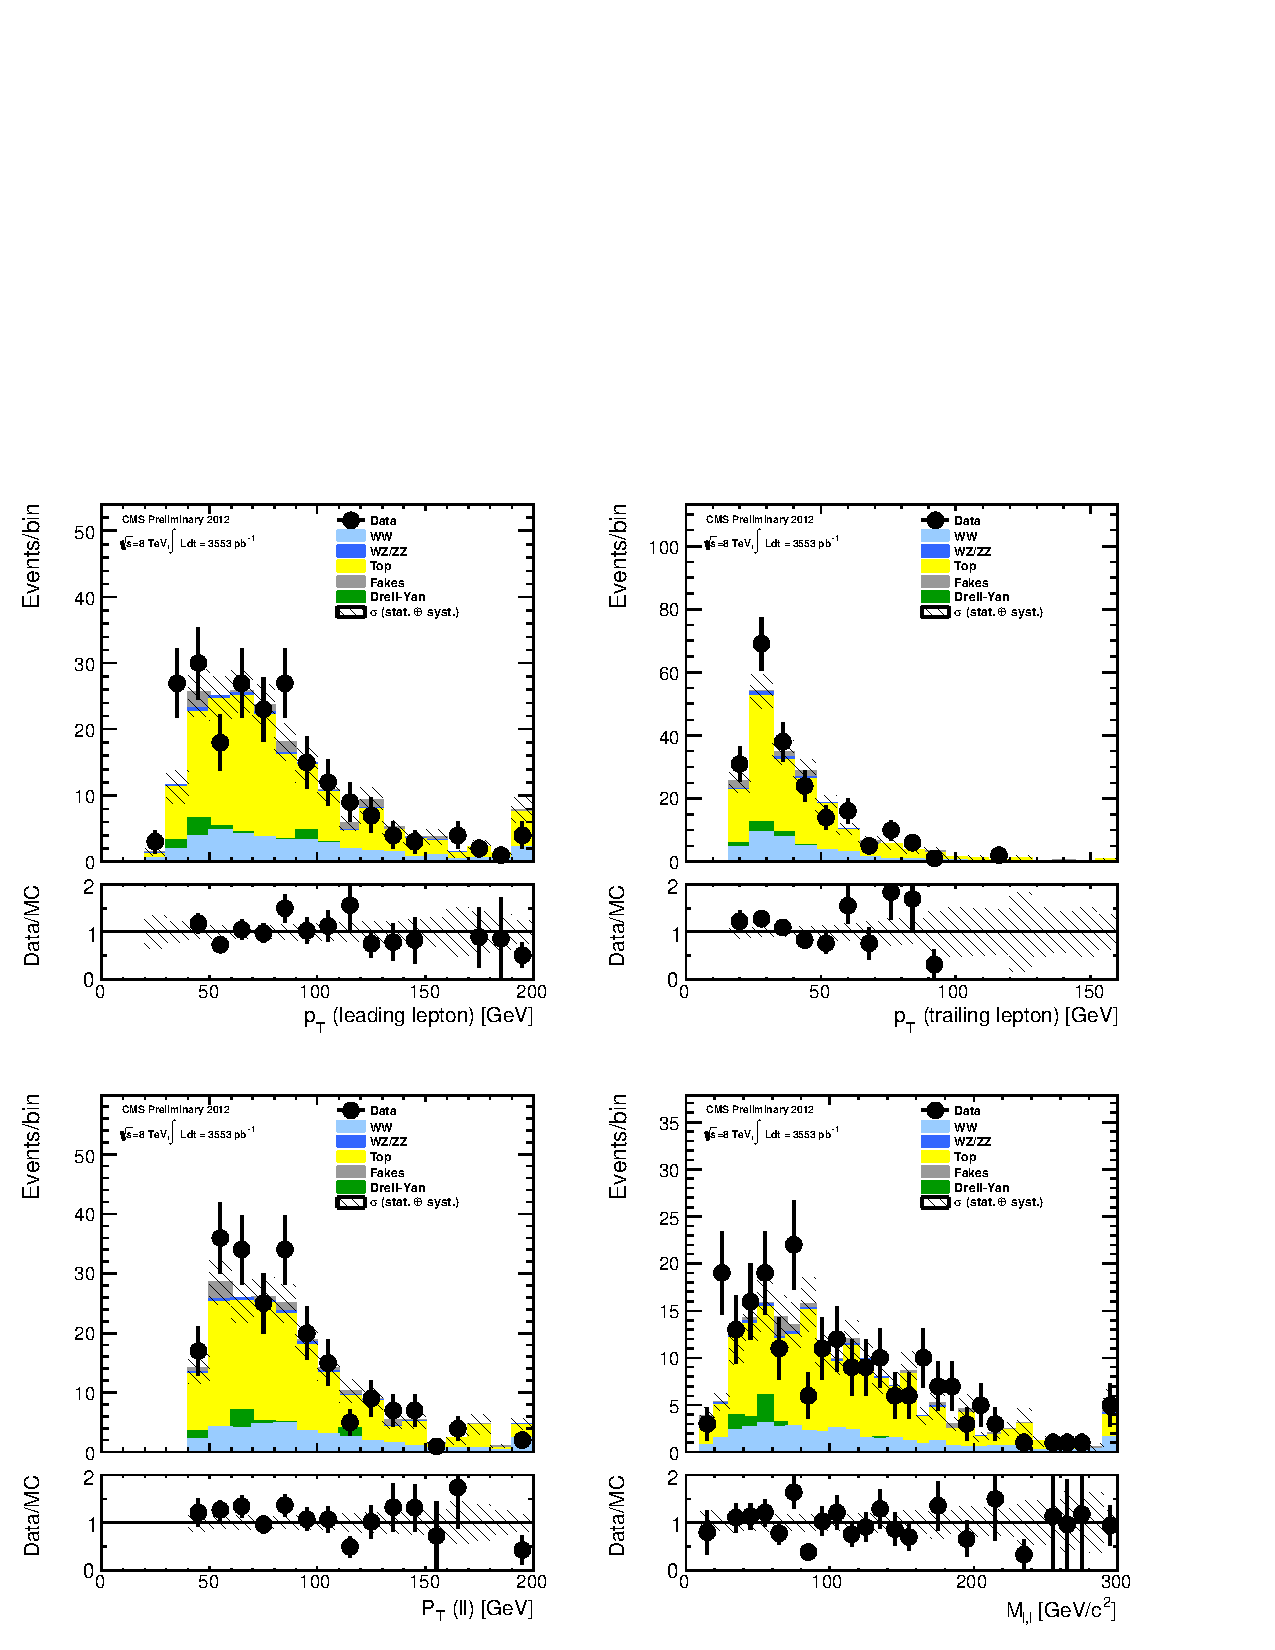
\includegraphics[width=1\textwidth]{figures/ww_analysis20_0_ALL_em_2j.pdf} %FIXME
\caption{Kinematic distributions in the $e\mu$ final state in the 2-jet bin.
The WW component has been scaled to the cross section measured in the 0-jet bin.}
\label{fig:xs_kinematics_em_2j}
\end{figure}
\begin{figure}[!hbtp]
\centering
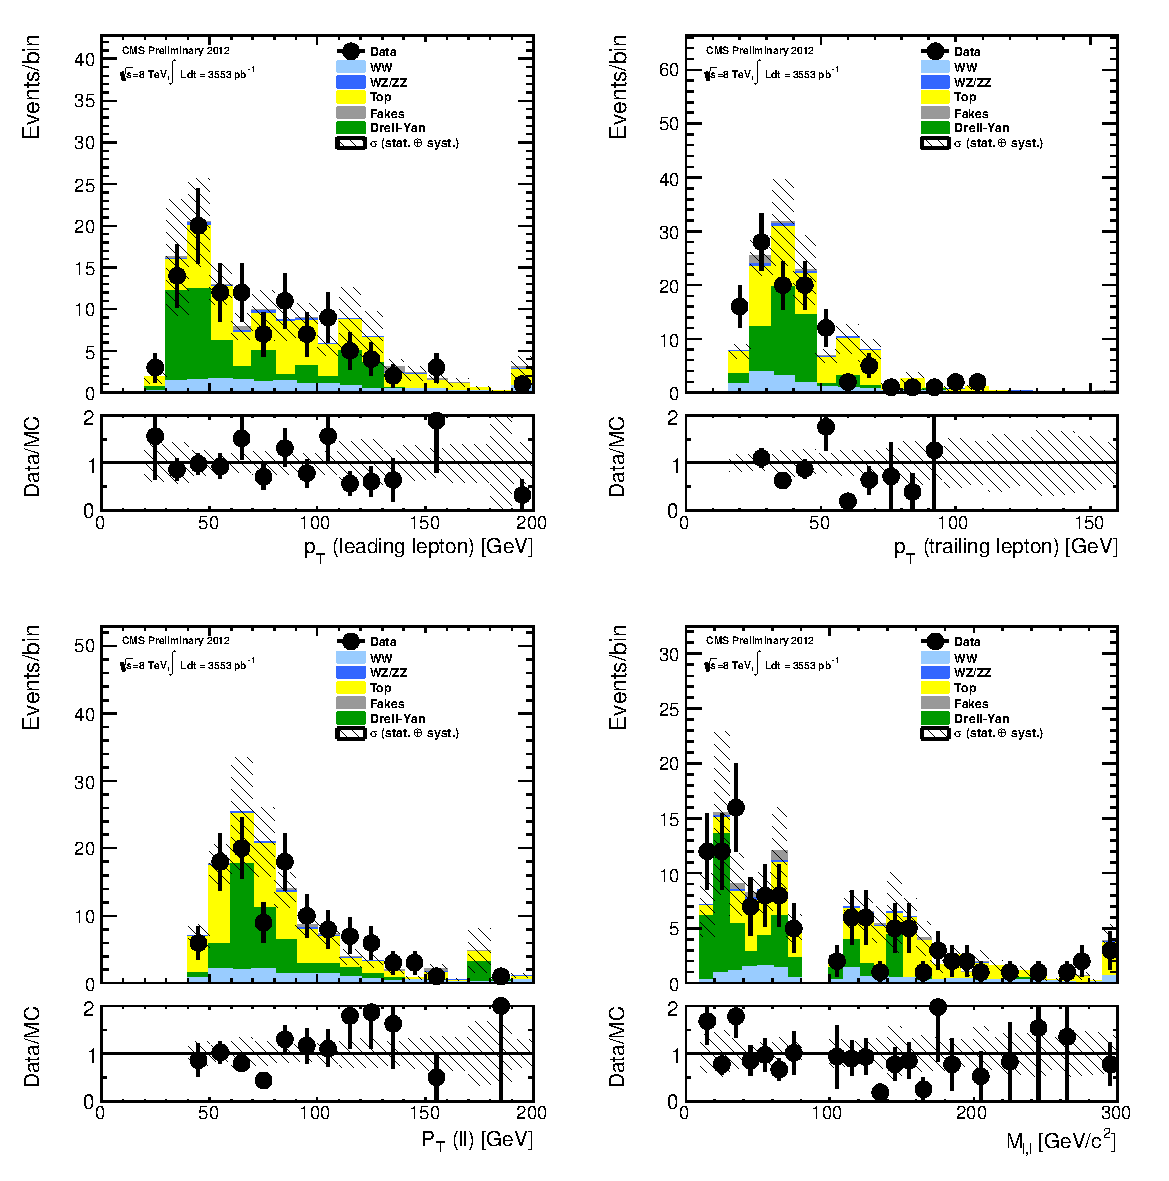
\includegraphics[width=1\textwidth]{figures/ww_analysis20_0_ALL_ee_2j.pdf} %FIXME
\caption{Kinematic distributions in the $ee$ final state in the 2-jet bin.
The WW component has been scaled to the cross section measured in the 0-jet bin.}
\label{fig:xs_kinematics_ee_2j}
\end{figure}
\begin{figure}[!hbtp]
\centering
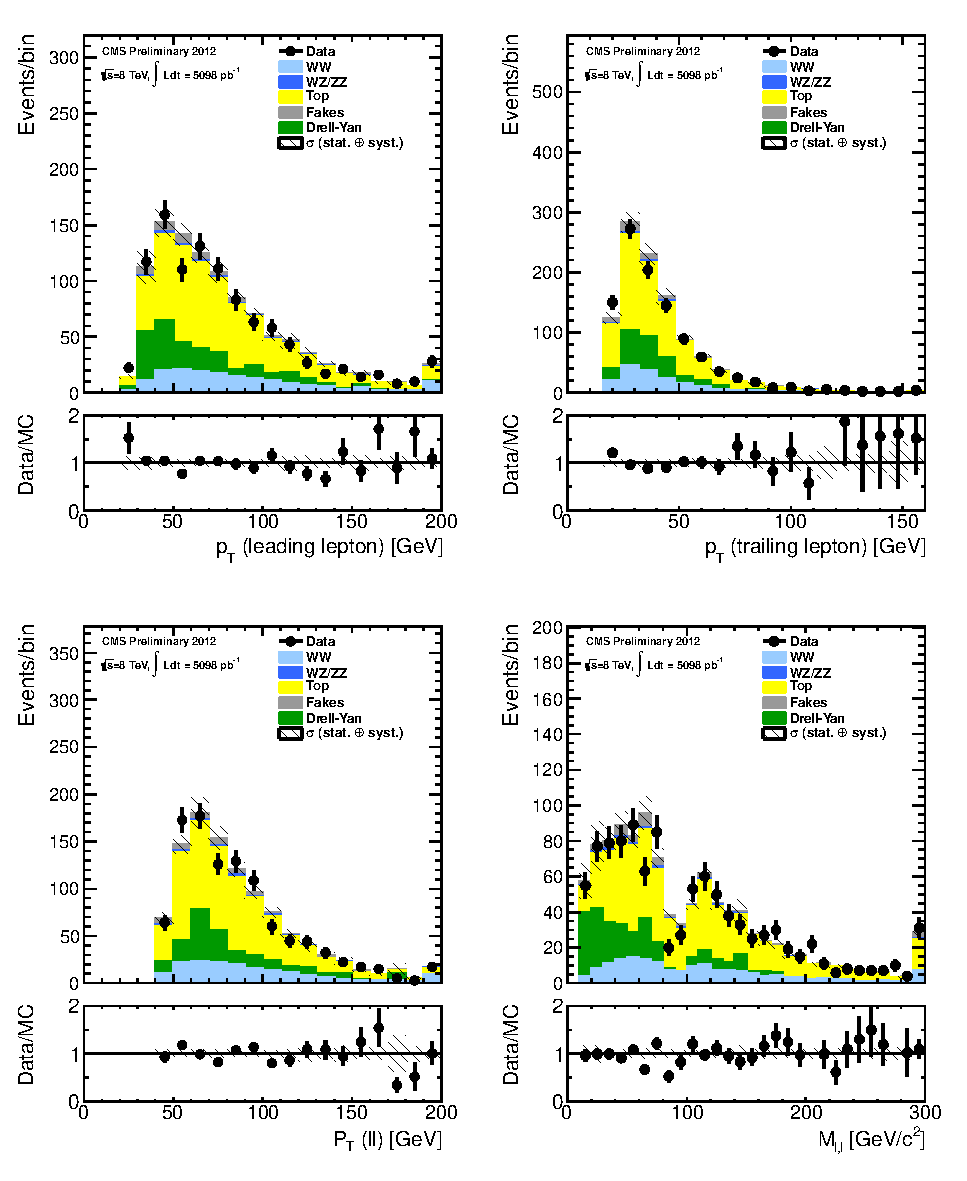
\includegraphics[width=1\textwidth]{figures/ww_analysis20_0_ALL_incl_2j.pdf} %FIXME
\caption{Kinematic distributions in the inclusive final state in the 2-jet bin.
The WW component has been scaled to the cross section measured in the 0-jet bin.}
\label{fig:xs_kinematics_incl_2j}
\end{figure}

\clearpage
\subsection{Summary}

The measurements in each jet bin and lepton channel are sumamrised in
Table \ref{tab:xs_summary}.  These are shown graphically 
in Figure \ref{fig:xs_summary_figure}.

\begin{table}[!ht]
\begin{center}
\begin{tabular}{|l|c|c|c|}
\hline
Channel              & 0-jet & 1-jet & 2-jet \\ \hline
$\sigma_{\mu\mu}$   &  $72.81\pm5.37\pm7.40\pm3.64$  & $79.97\pm13.83\pm13.45\pm4.00$ & $61.91\pm33.05\pm41.87\pm3.10$ \\
$\sigma_{\mu e}$   &  $74.03\pm4.45\pm6.49\pm3.70$  & $58.54\pm8.69\pm7.98\pm2.93$ & $72.89\pm20.98\pm17.39\pm3.64$ \\
$\sigma_{e \mu}$   &  $72.00\pm3.98\pm6.57\pm3.60$  & $65.41\pm8.06\pm8.48\pm3.27$ & $76.87\pm18.90\pm16.88\pm3.84$ \\
$\sigma_{ee}$   &  $47.77\pm5.99\pm7.12\pm2.39$  & $48.64\pm15.67\pm15.94\pm2.43$ & $22.62\pm38.16\pm56.17\pm1.13$ \\
\hline \hline
$\sigma_{tot.}$   &  $69.23\pm2.39\pm6.40\pm3.46$  & $63.77\pm5.18\pm8.21\pm3.19$ & $65.16\pm12.57\pm20.44\pm3.26$ \\
\hline
\end{tabular}
\caption{Summary of cross section results.  Uncertainties are $\mathrm{(stat.)} \pm \mathrm{(syst.)} \pm\mathrm{(lumi.)~pb}$.}
\label{tab:xs_summary}
\end{center}
\end{table}
\vspace{30pt}
\begin{figure}[!hbtp]
\centering
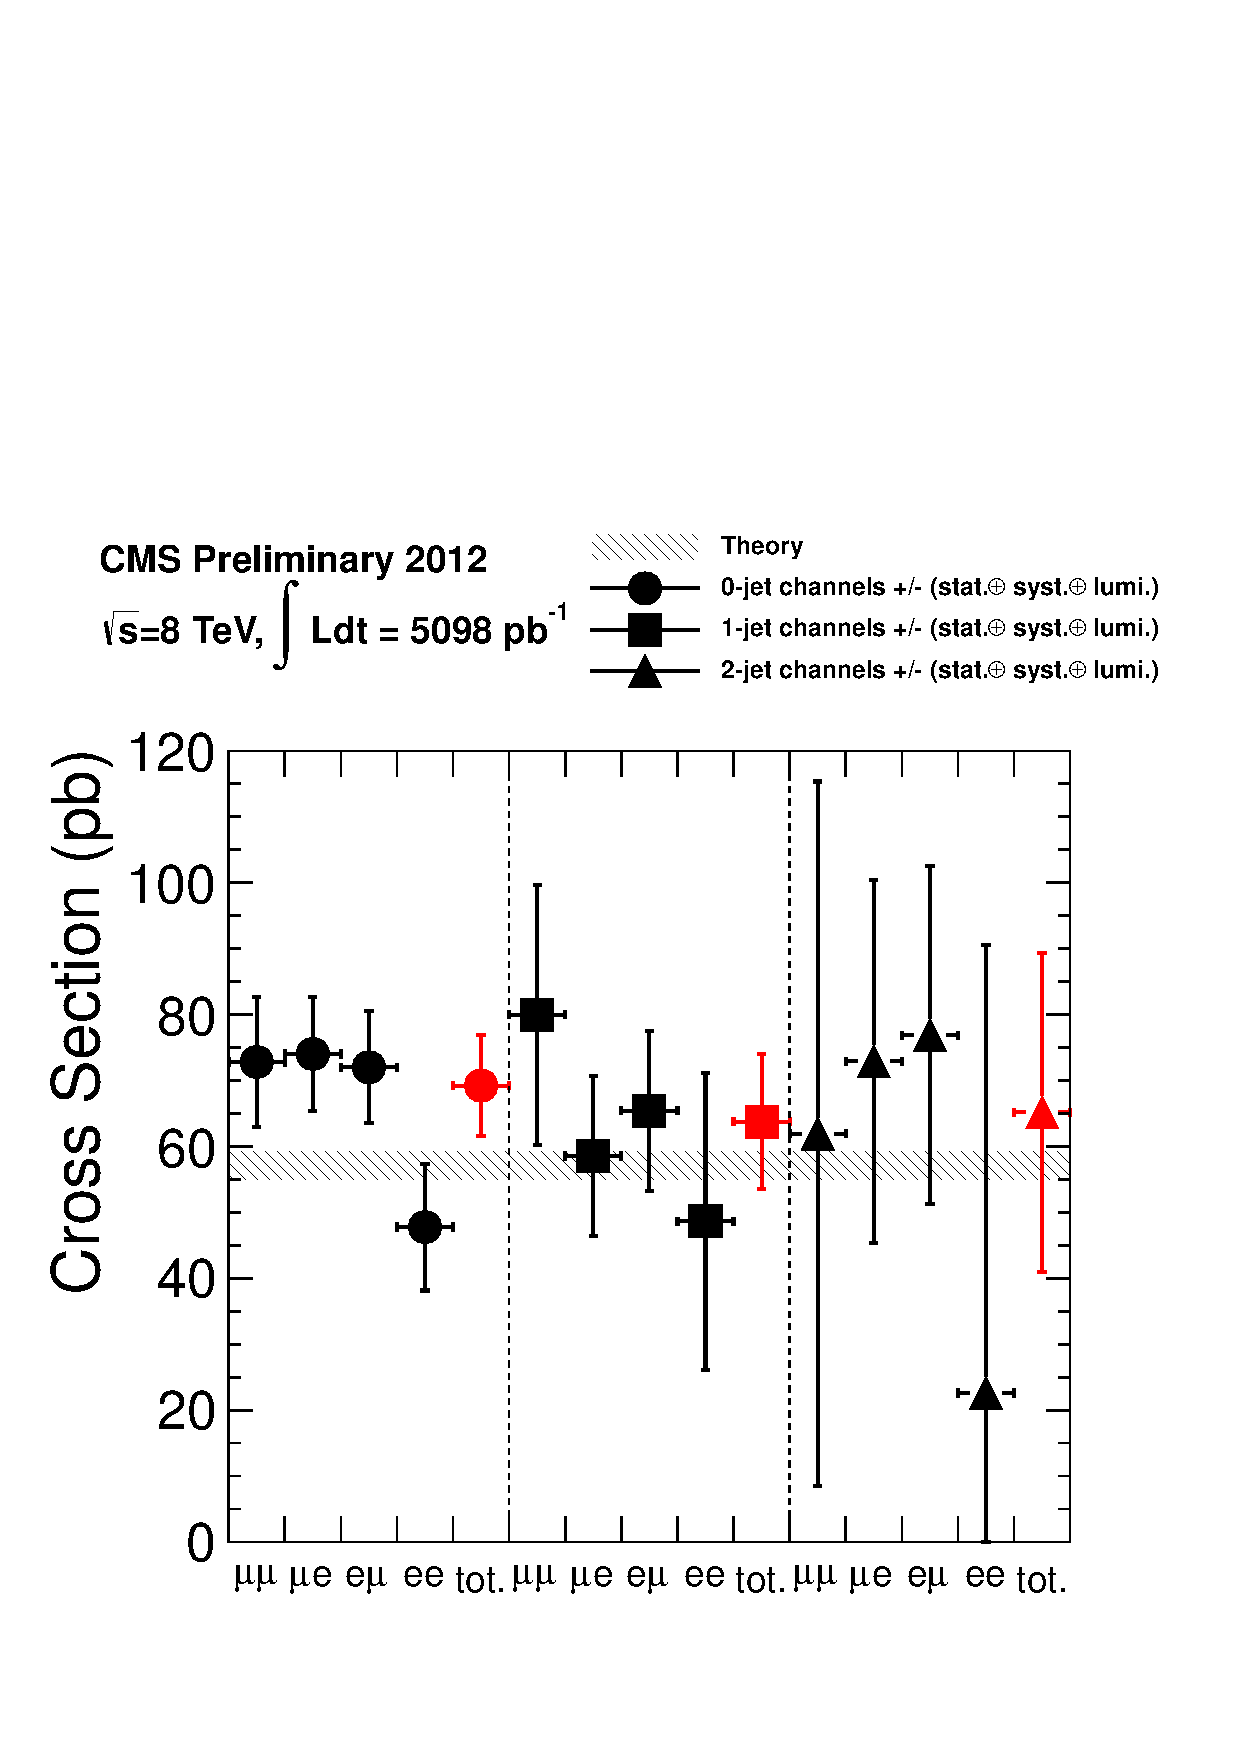
\includegraphics[width=.8\textwidth]{figures/ww_analysis20_0_summary.pdf} 
\caption{Summary of all channels. Total uncertainty is shown.}
\label{fig:xs_summary_figure}
\end{figure}




